\documentclass[11pt,mathserif]{beamer}
\usepackage{svg}
%% paketeak
\usepackage{amsmath,amssymb,amsfonts,amsthm}
\usepackage{graphicx}
\usepackage{bbding}
\usepackage{fontawesome}
\usepackage[utf8]{inputenc}
\usepackage[french]{babel}
\usepackage{fancyvrb}
\usepackage{relsize}
\usepackage{color}
\usepackage{listings}
\usepackage{caption}

% kolore batzuk definitu
\definecolor{dkgreen}{rgb}{0,0.6,0}
\definecolor{gray}{rgb}{0.5,0.5,0.5}
\definecolor{mauve}{rgb}{0.58,0,0.82}
\definecolor{bleuSympa}{rgb}{0.,0.19,0.607}
\definecolor{arrosa}{rgb}{0.7,0.15,0.15}

% bidexka erabilgarriak fontawesome erabiltzen
\newcommand{\scout}{\faAngellist}
\newcommand{\gezi}{\faLongArrowRight}
\newcommand{\galde}{\faQuestion}
\newcommand{\bof}{\faMehRollingEyes[regular]}
\newcommand{\hand}{\faHandORight}
\newcommand{\argi}{\faLightbulbO}
\newcommand{\Pdf}{\faFilePdfO}
\newcommand{\liburu}{\faBook}
\newcommand{\kontuz}{\faExclamationTriangle}
\newcommand{\pozik}{\faSmileO}
\newcommand{\triste}{\faFrownO}
\newcommand{\egia}{\faCheckCircle}

\captionsetup[figure]{labelformat=empty}

% listings kudeatzeko
\lstset{ %
  numbers=left,
  numbersep=1pt,
  numberstyle=\relsize{-5}\ttfamily,
  language=C,                % the language of the code
  framerule=1pt,
  basicstyle=\relsize{-3}\ttfamily,           % the size of the fonts that are used for the code
                                  % will be numbered
  %numbersep=5pt,                  % how far the line-numbers are from the code
  backgroundcolor=\color{black!20},      % choose the background color. You must add \usepackage{color}
  showspaces=false,               % show spaces adding particular underscores
  showstringspaces=false,         % underline spaces within strings
  showtabs=false,                 % show tabs within strings adding particular underscores
  %frame=single,                   % adds a frame around the code
  rulecolor=\color{black},        % if not set, the frame-color may be changed on line-breaks within not-black text (e.g. commens (green here))
  %tabsize=2,                      % sets default tabsize to 2 spaces
  breaklines=true,                % sets automatic line breaking
  breakatwhitespace=false,        % sets if automatic breaks should only happen at whitespace
  lineskip=-1pt,
  keywordstyle=\color{bleuSympa}\textbf,          % keyword style
  commentstyle=\color{bleuSympa},       % comment style
  stringstyle=\color{mauve},
  emph={ __global__, __shared__, __device__, __host__,
        __syncthreads, threadIdx, blockIdx, blockDim},
  emphstyle=\color{arrosa},
  moredelim=[s][\color{arrosa}\ttfamily]{<<<}{>>>},
  morecomment=[s][\color{mauve}]{cudaMemcpyHostToDevice}{\ },
  morecomment=[s][\color{mauve}]{cudaMemcpyDeviceToHost}{\ }
}


\defbeamertemplate{itemize item}{boldarrow}{\raisebox{0.3ex}{\resizebox{1.2ex}{1ex}{\ArrowBoldRightShort}}}

%% ====== nire beamer estiloa
\mode<presentation> {
\usetheme{default}    % urri
\useinnertheme[shadow]{rounded}  % zenbakiak biribiltzeko
}
\usefonttheme{structurebold}

\begin{document}

%****************************************************************
% Aurkezpen orria
%**************************************************************
\begin{frame}
\begin{center}
  {\Large Une introduction au calcul sur GPU (I) } 
\end{center}
\begin{center}
\includegraphics[width=0.5\linewidth]{fig/gpu.jpg}
\end{center}
\begin{center}
{\large Marc Fuentes - INRIA Pau\\ }
\end{center}
\end{frame}

%****************************************************************
% Xedea
%**************************************************************

\begin{frame}{Plan}
\begin{itemize}[<+->]
\item Exemple d'applications 
\item Prolégomènes (parallèlisme, mémoire, cache)
\item Exemple d'introduction
\item Modèle d'exécution d'un GPU
\item Accès mémoires et coalescence
\item Outils (déverminage, profilage)
\end{itemize}
\end{frame}
%****************************************************************
% Applications
%**************************************************************

\begin{frame}{Utilisation des GPU}
\pause
  \begin{itemize}[<+->]
    \item 
      \begin{minipage}[c]{0.49\linewidth}
        calcul haute performance (HPC) : simulation numérique de grande taille
      \end{minipage}
      \begin{minipage}[c]{0.49\linewidth}
        \begin{figure}
        \includegraphics[width=0.6\linewidth]{fig/titan.jpg}
          \caption{\tiny Supercalculateur Titan : $\thicksim$ 18000 GPU }
        \end{figure}
      \end{minipage}
    \item  \begin{minipage}[l]{0.49\linewidth}
     traitement d'image, jeux vidéos 
      \end{minipage}
      \begin{minipage}[r]{0.49\linewidth}
        \begin{figure}
        \includegraphics[width=0.6\linewidth]{fig/minetest.jpg}
          \caption{\tiny Minetest (clone libre) }
        \end{figure}
      \end{minipage}
    \item  \begin{minipage}[l]{0.49\linewidth}
     apprentissage automatique
      \end{minipage}
      \begin{minipage}[r]{0.49\linewidth}
        \begin{figure}
        \includegraphics[width=0.6\linewidth]{fig/neural.png}
          \caption{\tiny véhicule autonome(projet inutile \faMehO)}
        \end{figure}
      \end{minipage}
  \end{itemize}
\end{frame}

%****************************************************************
% Parallèlisme Distribue/partagé
%****************************************************************
\begin{frame}{Parallèlisme}{partagé/distribué}
\pause
La mémoire utilisée peut être distribuée ou partagée.
  \begin{itemize}[<+->]
    \item mémoire partagée : on a des threads (fils d'exécution) ou tâches qui accèdent à une mémoire commune. 
      \begin{itemize}
        \item[\pozik] rapidité d'accés en lecture/écriture
        \item[\kontuz] accés concurrents : utilisation de verrous ou d'opérations atomiques
        \item[\argi] cibles : Threads Posix, OpenMP, CUDA
      \end{itemize}
    \item mémoire distribuée : chaque processus a une mémoire privée et communique avec les autres par des messages
      \begin{itemize}
        \item[\argi] nécéssaire sur de trés grand problème (limite mémoire/nœud  moins gênante)
        \item[\triste] envoie de messages peut être couteux
        \item[\argi] cibles : MPI, Multi-GPU
      \end{itemize}
  \end{itemize}
\end{frame}
%****************************************************************
% Parallèlisme : Grain
%****************************************************************
\begin{frame}{Parallèlisme}{Grain}
\begin{itemize}[<+->]
  \item gros grain : un processeur parallèle (tâche, threads, processus MPI) traite beaucoup d'éléments 
   \begin{itemize}
     \item décomposition de domaine (maillage, matrice) :  ex. MUMPS
     \item parallèlisme par tâches avec support d'execution (ex : STARPU)
     \item chaque processeur doit avoir suffisament de mémoire pour traiter une grosse tâche
   \end{itemize}
   \item grain fin : chaque processeur traite une «donnée élémentaire»
   \begin{itemize}
     \item[\kontuz] nécessite un grand nombre de threads
     \item[\kontuz] le changement de contexte doit être négligeable
   \end{itemize}
\end{itemize}
\end{frame}
%****************************************************************
% Parallèlisme : architecture
%****************************************************************
\begin{frame}{Parallèlisme}{Architecture}
\begin{itemize}[<+->]
  \item homogène : processeurs quasi-identiques ou de caractéristiques semblables(latence, mémoire, etc)
   \begin{itemize}
     \item processeurs vectoriels (Cray, DEC)
     \item modèle SIMD : Single Instruction Multiple Data (MMX, SSE, AVX)
     \item grappe de calcul MPI avec des nœuds identiques
   \end{itemize}
  \item hétérogène : on observe des disparités entre les différents processeurs
   \begin{itemize}
     \item Calcul sur GPU : hôte vs accélérateur
     \item Processeur Cell dans les PS3
   \end{itemize}
\end{itemize}
\pause
  \hand La programmation sur GPU est {\it grosso modo}\  donc un parallèlisme à {\bf grain fin}, à mémoire {\bf partagée} tournant sur
  une architecture {\bf hétérogène}.
\end{frame}

%****************************************************************
% Prolègomène II
%****************************************************************
\begin{frame}{Mémoire et Cache}{schéma}
\begin{itemize}[<+->]
  \item La rapidité d'exécution d'un calcul dépend aussi de la «proximité» avec le CPU de l'élément de mémoire à traiter 
  \item[\gezi] les concepteurs de CPU ont créé des {\bf caches} pour stocker les valeurs mémoires les plus utilisées
  \begin{center}
    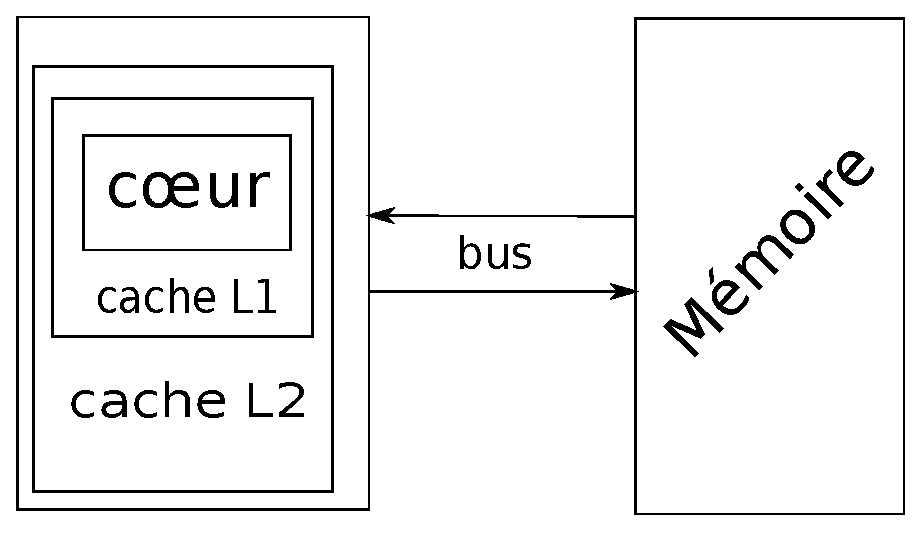
\includegraphics[width=0.7\linewidth]{fig/cpu_classique.eps}
  \end{center}
\end{itemize}
\end{frame}
%****************************************************************
% Prolegomenes III
%****************************************************************
\begin{frame}{Mémoire et Cache (II)}{latence}
\pause
  \begin{itemize}[<+->]
  \item ainsi la latence $l$ de l'emplacement mémoire auquel on accède  respecte
  $$l({\mbox{\scriptsize registre}}) \leqslant l(\mbox{\scriptsize cache L1}) \leqslant
    l(\mbox{\scriptsize cache L2}) \leqslant l(\mbox{\scriptsize mémoire globale}).$$
  \item ordres de grandeur des latences (core i7 Xeon E5500)
    \begin{tabular}{|l|c|c|}
    \hline
      type & nb cycles & latence (ns)  \\
    \hline
      cache L1  &  4 & 2 \\
      cache L2  &  10 & 5 \\
      cache L3 (non partagé) & 40 & 20  \\
      cache L3 (partagé) &  65 & 35  \\
      mémoire vive locale & & 60 \\
      mémoire vive distante & & 100 \\
    \hline
    \end{tabular}
  \end{itemize}
\end{frame}
%%****************************************************************
%% Prolegomenes IV
%%****************************************************************
\begin{frame}{Cache : Succès et défauts}
\begin{itemize}[<+->]
 \item succès (hit): accès à un emplacement présent dans la ligne de cache 
 \item défaut (miss) : accès hors de la ligne de cache $\rightarrow$ il faut recharger entierement la ligne de cache!
 \item un code localisant ses accès dans le cache minimise les défauts de cache et tourne plus vite
 \item ex. double boucle en C sur les lignes (resp. colonnes en Fortran)
\end{itemize}
\pause
\begin{minipage}[c]{0.49\linewidth}
  \lstinputlisting[language=C]{code/loop_col.c}
\end{minipage}
\begin{minipage}[c]{0.49\linewidth}
    \begin{tabular}{|c|c|}
    \hline
     boucle ext. & tps(s)  \\
    \hline
      i (lignes) & 2.7s \\
      j (cols)  & 3.4s \\
    \hline
    \end{tabular}
\end{minipage}
\pause 
 $\Rightarrow$ raison d'être des biblios BLAS et LAPACK
\end{frame}
%%****************************************************************
%% Prolegomenes V
%%****************************************************************
%%%\begin{frame}{Passage à l'échelle}
%%%\begin{itemize}[<+->]
%%%  \item fort (strong scalability)
%%%    \begin{itemize} 
%%%       \item loi d'Amdhal (pessimiste)
%%%    \end{itemize}
%%%  \item faible (weak scalability)
%%%    \begin{itemize}
%%%      \item loi
%%%    \end{itemize}
%%%\end{itemize}
%%%\end{frame}
%%****************************************************************
%% Exemple introductif (séquentielle)
%%****************************************************************
\begin{frame}{Exemple d'introduction}{version séquentielle}
\pause
\begin{itemize}[<+->]
 \item soit un programme calculant \texttt{tab[:]} $\leftarrow$ \texttt{tab[:] + 3}
\lstinputlisting{code/increment.c}
\item on souhaite paralléliser la boucle en ligne 6 à l'aide de CUDA
\end{itemize}
\end{frame}
%%****************************************************************
%% Exemple introductif (CUDA)
%%****************************************************************
\begin{frame}{Exemple d'introduction}{version CUDA}
\pause
\begin{itemize}[<+->]
 \item on peut écrire le programme suivant
\lstinputlisting{code/incrementGPU.cu}
\item plus de boucle!
\item nouveaux mot-clefs : \texttt{\_\_global\_\_, threadIdx}
\item appel du noyau \texttt{increment<<<1,N>>>}
\item gestion de la mémoire : \texttt{cudaMemcpy, cudaMalloc, cudaFree}
\end{itemize}
\end{frame}
%****************************************************************
% Exemple introductif principe
%****************************************************************
\begin{frame}{Exemple d'introduction}{explication}
\pause
\begin{itemize}[<+->]
 \item boucle \alert{for} $\rightarrow$ appel d'un {\bf thread}
 \item qui exécute le noyau \alert{increment}
 \item pour chaque indice de boucle : \lstinline!threadIdx.x!
 \item sur le tableau \alert{tab\_d} alloué sur le GPU
 \item il faut copier \alert{tab} sur le GPU et le rapatrier après calcul
\end{itemize}
\pause
\begin{center}
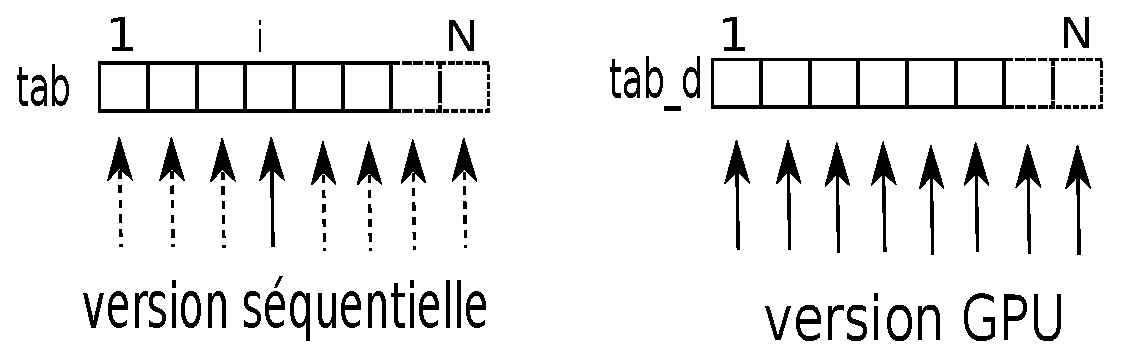
\includegraphics[width=0.9\linewidth]{fig/parallel.eps}
\end{center}
\end{frame}
%****************************************************************
% Déroulé classique d'un calcul
%****************************************************************
\begin{frame}{Déroulé typique d'un calcul}
  \lstset{basicstyle=\ttfamily}
\pause
  \begin{itemize}[<+->]
  \item un programme CUDA suit généralement les étapes suivantes 
\begin{enumerate}[<+->]
 \item allouer la mémoire sur le GPU : \lstinline!cudaMalloc!
 \item copier depuis la mémoire globale vers le GPU : \lstinline!cudaMemCpy( ... ,cudaMemcpyHostToDevice)!
 \item exécuter le noyau sur l'accélerateur : \lstinline!myKernel<<<...,...>>>(...)!
 \item rapatrier les résultats en mémoire globale \lstinline!cudaMemCpy(...,cudaMemcpyDeviceToHost)!
 \item libérer la mémoire sur le GPU \lstinline!cudaFree!
 \item visualiser les résultats
\end{enumerate}
\item Avant de poursuivre, nous avons besoin de comprendre le modèle d'exécution sur GPU
\end{itemize}
\end{frame}
%****************************************************************
% Modèle d'execution GPU I
%****************************************************************
\begin{frame}{Modèle d'exécution du GPU}{exemple sur un Tesla C1060}
\begin{minipage}[c]{0.49\linewidth}
\begin{itemize}
  \item multiprocesseur de flux (SM)
    \begin{itemize}
      \item groupe de 8 processeurs de flux (SP)
        \begin{itemize}
          \item partage de mémoire locale
          \item synchronisation
        \end{itemize}
    \end{itemize}
  \item processeur de flux (SP) : 
    \begin{itemize}
    \item 64KB de registres, 
    \item {\bf threads} : ensemble de registres
    \begin{itemize}
      \item création/destruction gratuites
    \end{itemize}
  \item exécution entrelacée de {\em threads} matériels : jusqu'à 128 par SP
    \end{itemize}
\end{itemize}
\end{minipage}
\begin{minipage}[c]{0.49\linewidth}
\begin{center}
  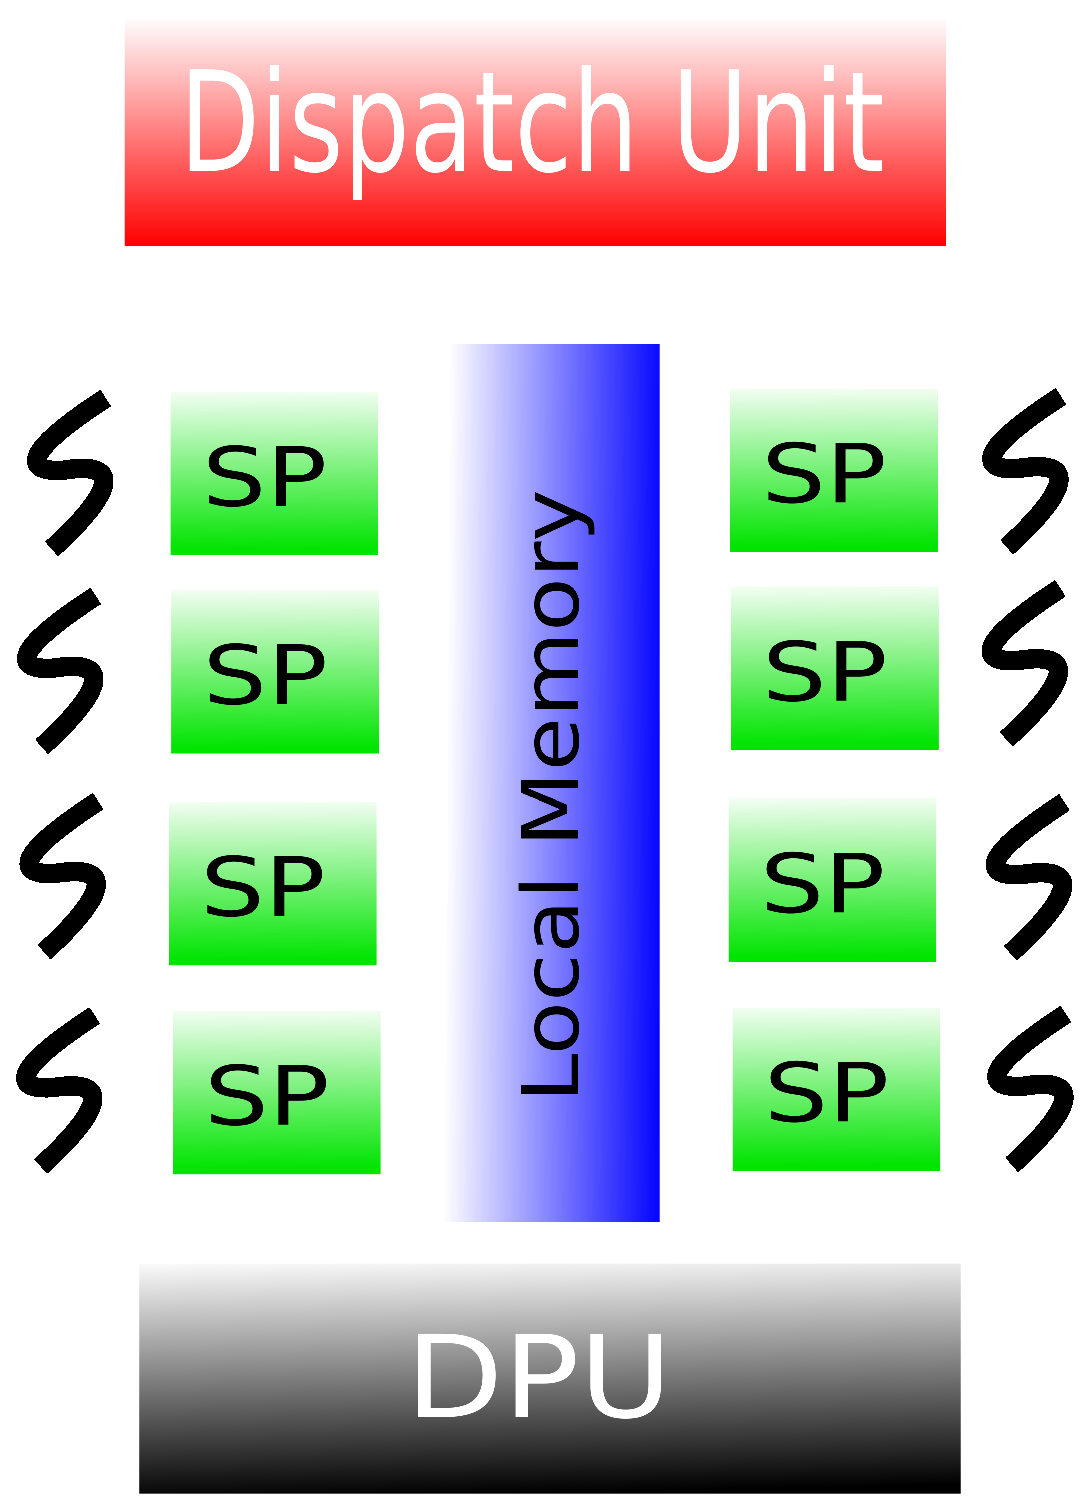
\includegraphics[width=0.6\linewidth]{fig/GPUArchiThread.eps}
\end{center}
\end{minipage}
\end{frame}
%****************************************************************
% Modèle d'execution GPU II
%****************************************************************
\begin{frame}{Modèle d'exécution du GPU}{exemple sur un Tesla C1060 (II)}
\begin{minipage}[c]{0.49\linewidth}
\begin{itemize}
  \item 1 seule unité d'envoi d'instruction par multiprocesseur de flux
    \begin{itemize}
      \item tous les SP exécutent la même instruction au même cycle d'horloge
        \begin{itemize}
          \item sur des données différentes (SIMD)
        \end{itemize}
    \end{itemize}
  \item l'unité d'envoi prend 4 cycles pour récupérer et décoder les instructions
    \begin{itemize}
      \item 4 groupes de 8 {\bf threads} planifiés / ligne
    exécutant la même instruction
      \item changement de contexte gratuit !
    \end{itemize}
\end{itemize}
\end{minipage}
\begin{minipage}[c]{0.49\linewidth}
\begin{center}
  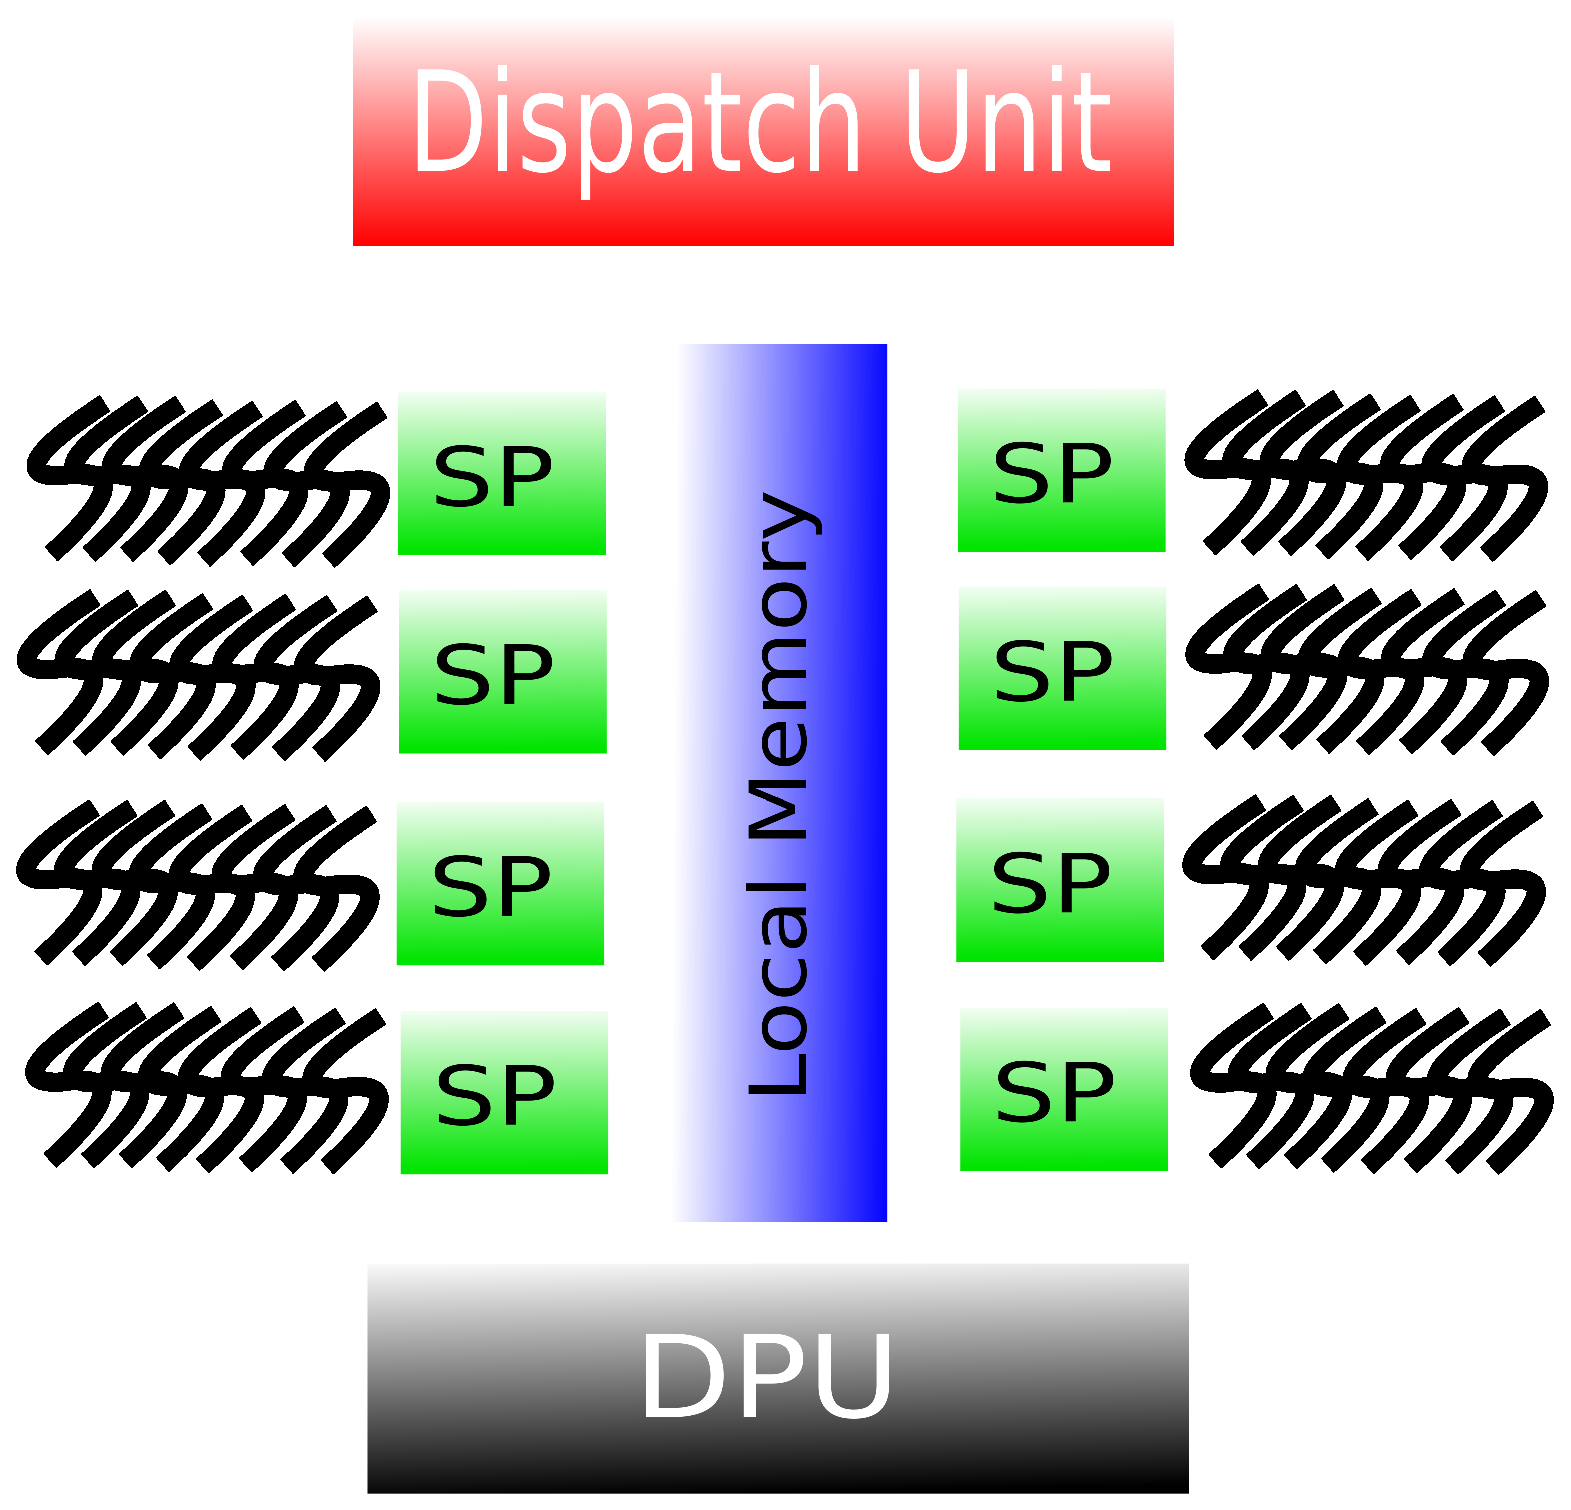
\includegraphics[width=0.9\linewidth]{fig/GPUArchi8Thread.eps}
\end{center}
\end{minipage}
\end{frame}
%****************************************************************
% Modèle d'execution GPU III
%****************************************************************
\begin{frame}{modèle d'exécution du GPU}{warps et demi-warps}
\begin{minipage}[c]{0.59\linewidth}
\begin{itemize}
  \item les {\bf threads} sont implicitement groupés en {\bf warps}
    \begin{itemize}
      \item un {\bf warp} (chaîne) = 32 threads 
      \item tous les threads d'une même chaîne exécutent la même instruction au même cycle logique
        \begin{itemize}
          \item[\kontuz] \alert{pas de divergence!}
        \end{itemize}
    \end{itemize}
  \item charger des données depuis la mémoire globale est coûteux
    \begin{itemize}
      \item plus de 4 threads nécessaires / SP
      \item 128 permettent de recouvrir la latence mémoire
    \end{itemize}
\end{itemize}
\end{minipage}
\begin{minipage}[c]{0.39\linewidth}
\begin{center}
  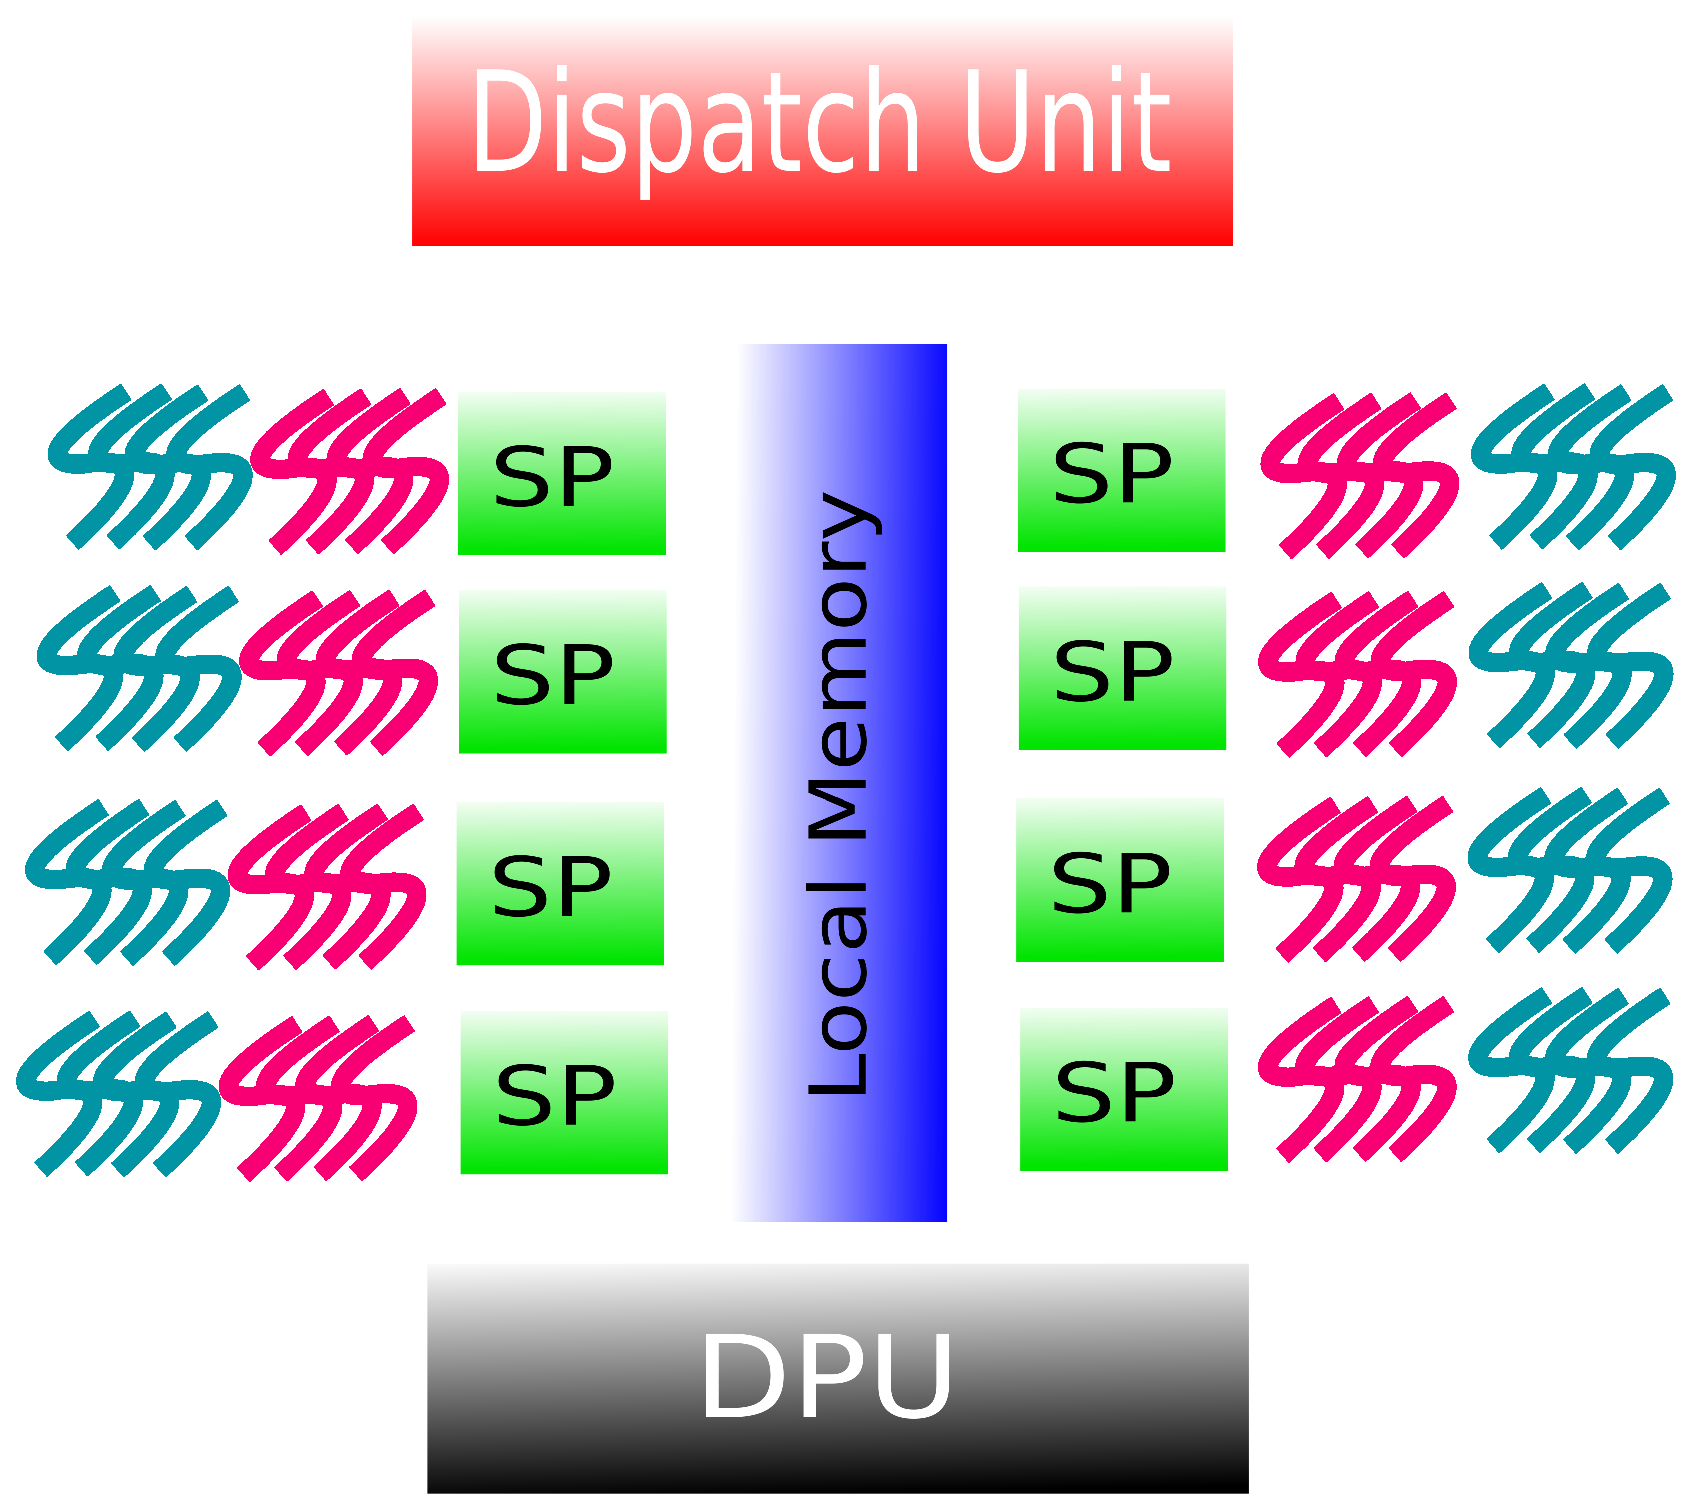
\includegraphics[width=0.95\linewidth]{fig/GPUArchi8ThreadDiv.eps}
\end{center}
\end{minipage}
\end{frame}
%****************************************************************
% Modèle d'execution GPU IV
%****************************************************************
\begin{frame}{modèle d'exécution du GPU}{exemple avec un K40M}
\begin{minipage}[c]{0.59\linewidth}
  \begin{itemize}[<+->]
    \item GPU = ensemble de multiprocesseurs de flux (SM) partageant une mémoire globale (DRAM)
    \item Tesla K40M : 
      \begin{itemize}
        \item 15 SM, 192 SP / SM $\Rightarrow$ 2880 SP
        \item 2048 threads max / SM $\Rightarrow$ 30.720 threads
      \end{itemize}
    \item threads «speciaux»
      \begin{itemize}
        \item parallélisme de données respectant des motifs d'accès réguliers
      \end{itemize}
  \end{itemize}
\end{minipage}
\begin{minipage}[c]{0.39\linewidth}
\begin{center}
  \rotatebox{90}{\includegraphics[width=0.9\linewidth]{fig/kepler.jpg}}
\end{center}
\end{minipage}
\end{frame}
%****************************************************************
% Organisation des threads
%****************************************************************
\begin{frame}{Organisation des threads}{découpage des données}
 \pause
 \begin{minipage}[c]{0.59\linewidth}
  \begin{itemize}[<+->]
    \item K40M $\approx$ 30K threads 
    \item Que faire si $N \geq 30K$ ?
    \item on découpe les données en blocs
    \item threads organisés en \alert{blocs} qui tournent chacun sur 1 SM
    \item une \alert{grille} répartie les blocs sur tous les SMs
    \item on paramètre l'appel du noyau \lstinline!myKernel<<<grille,blocs>>>(...)! avec la taille des blocs et de la grille (int ou dim3)
  \end{itemize}
\end{minipage}
\begin{minipage}[c]{0.39\linewidth}
\begin{center}
  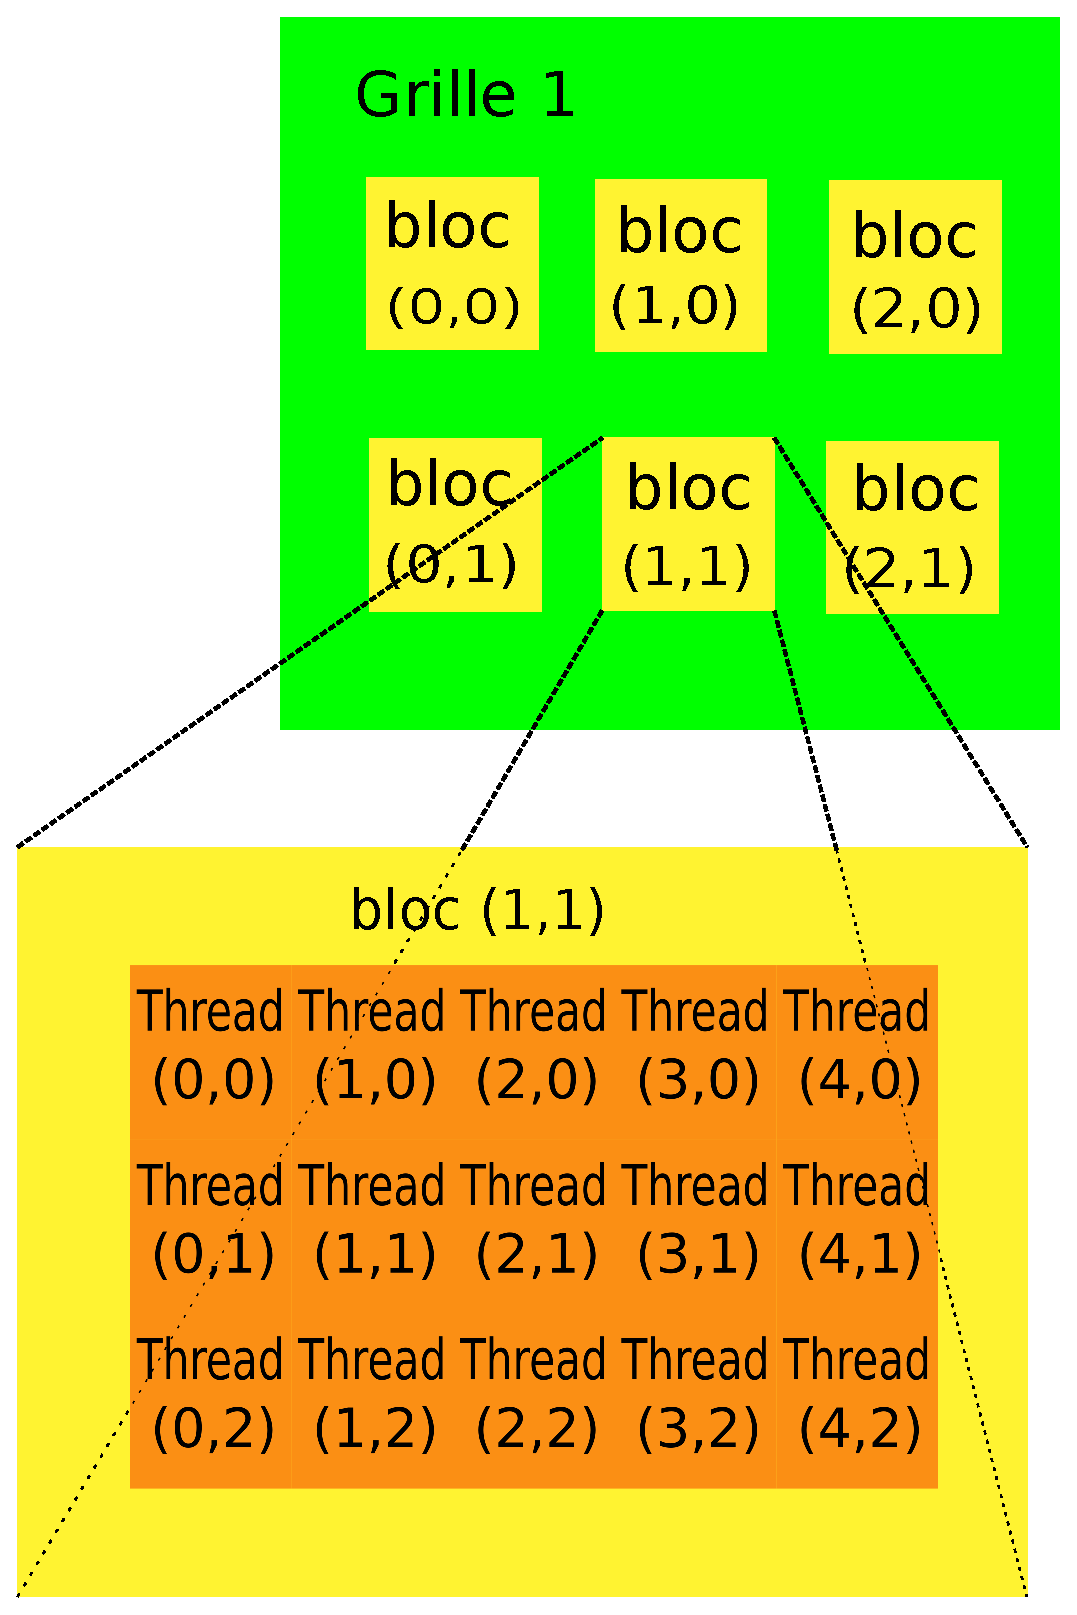
\includegraphics[width=0.8\linewidth]{fig/grille_et_blocs.eps}
\end{center}
\end{minipage}
\end{frame}
%****************************************************************
% Organisation des threads II
%****************************************************************
\begin{frame}{Organisation des threads}{ordonnancement}
 \pause
 \begin{minipage}[c]{0.59\linewidth}
   {\bf Le programme sur l'hôte demande l'exécution d'une grille de blocs de threads}
  \begin{itemize}[<+->]
    \item l'ordonnanceur de bloc distribue les blocs sur les SMs
    \item[\kontuz] des GPUs différents peuvent exécuter différemment la même grille de blocs
  \end{itemize}
\end{minipage}
\begin{minipage}[c]{0.39\linewidth}
\begin{center}
  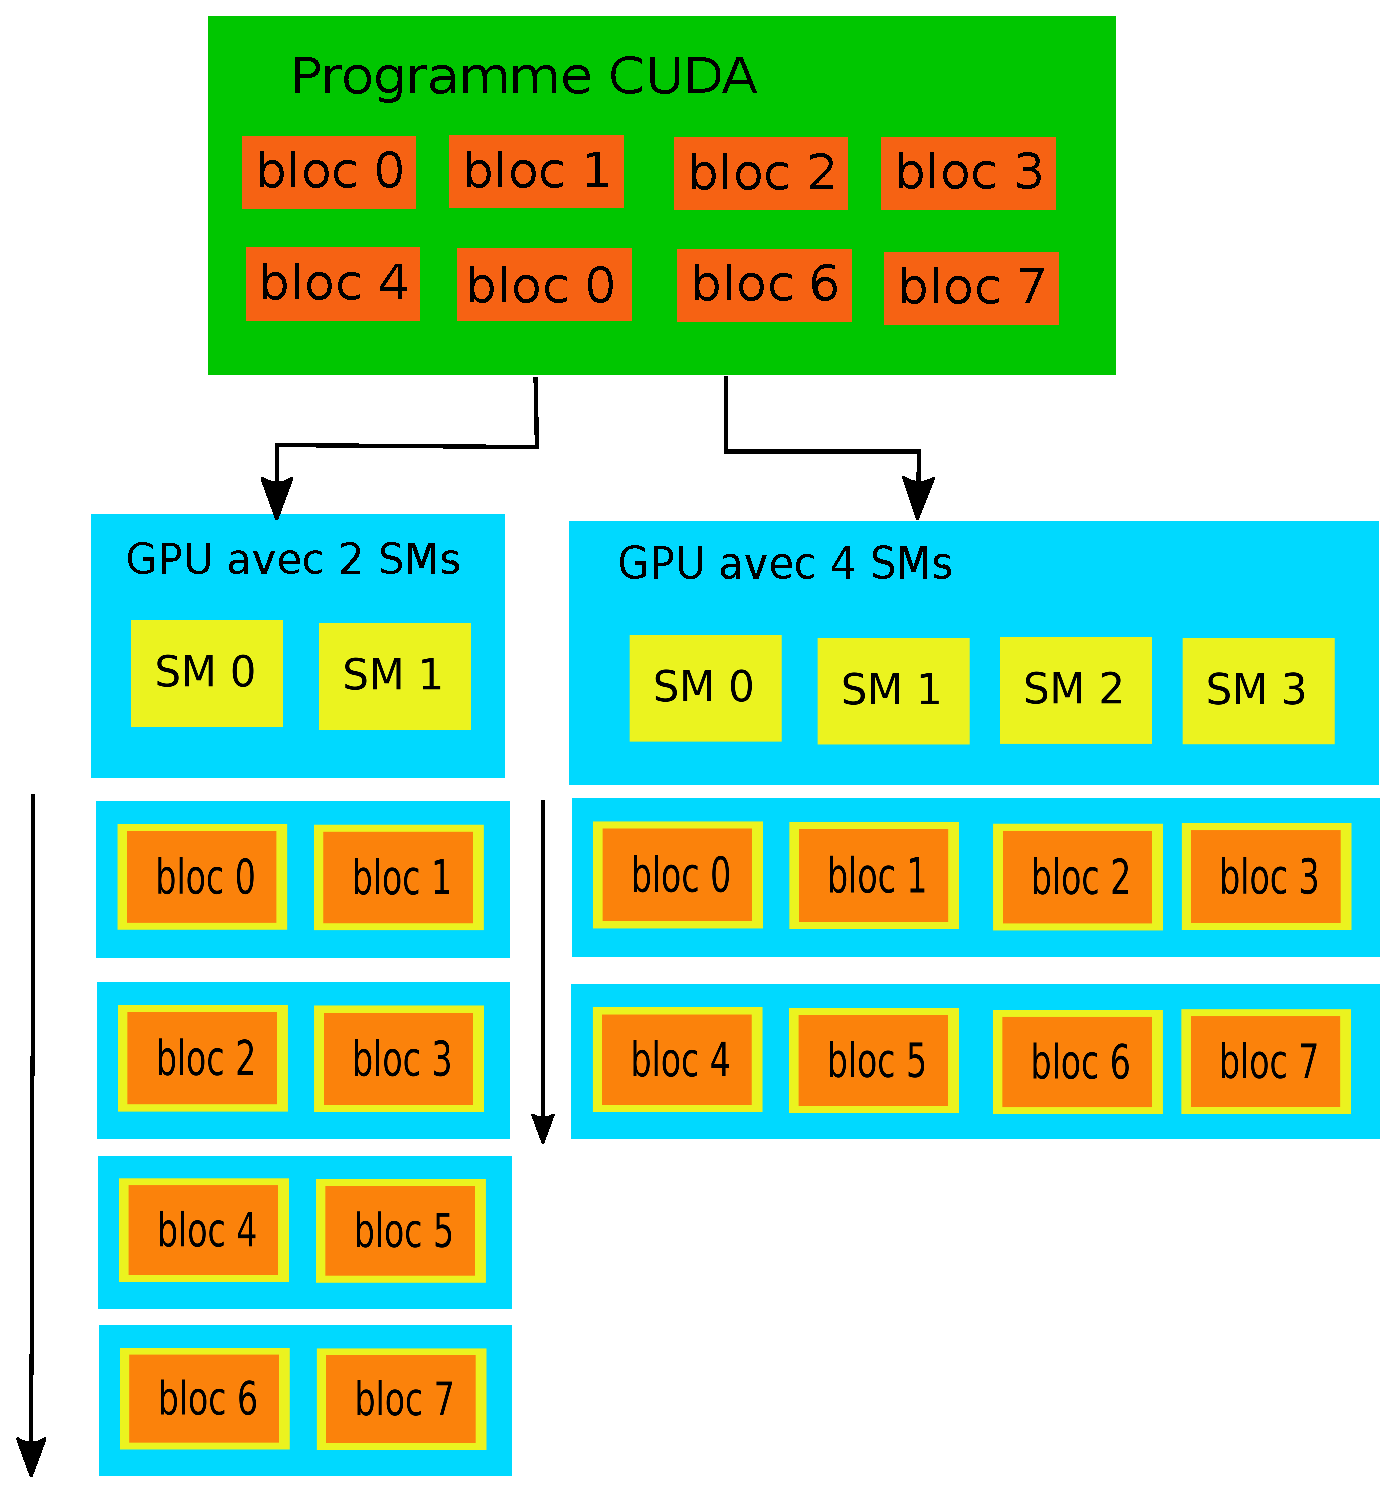
\includegraphics[width=0.95\linewidth]{fig/bloc_ordonanceur.eps}
\end{center}
\end{minipage}
\end{frame}
%****************************************************************
% Tailles des grilles/blocs 
%****************************************************************
\begin{frame}{Tailles de grille et de blocs}
  \begin{itemize}[<+->]
    \item type CUDA pour gérer les dimensions de grille et de bloc
    \begin{itemize}
      \item \alert{dim3} est une structure avec 3 champs entiers \texttt{\_.x,\_.y et \_.z}
      \item soit \texttt{dg} un descripteur de grille et \texttt{db} un descripteur de bloc
    \end{itemize}
  \item Limites de bloc 3D
   \begin{itemize}
     \item \texttt{db.x} $\leqslant 1024$, \texttt{db.y} $\leqslant 1024$, \texttt{db.z} $\leqslant 64$ 
     \item nb total de threads par bloc $\leqslant 1024$
     \item problèmes 2D \gezi\  \texttt{db.z} = 1 
     \item problèmes 1D \gezi\  \texttt{db.z} = \texttt{db.y} = 1
   \end{itemize}
 \item limites de la grille 3D
   \begin{itemize}
     \item \texttt{dg.x} $\leqslant 2^{31}-1$, \texttt{dg.y} $\leqslant 2^{16} - 1 $, \texttt{dg.z} $\leqslant 2^{16}-1$
     \item nb total de threads par bloc $\leqslant 1024$
     \item problèmes 2D \gezi\  \texttt{dg.z} = 1 
     \item problèmes 1D \gezi\  \texttt{dg.z} = \texttt{dg.y} = 1
  \end{itemize}
 \item exemple avec données 2D mais une grille 1D
  \lstinputlisting[language=C]{code/grille.c}
 \end{itemize}
\end{frame}
%****************************************************************
% Tailles des grilles/blocs
%****************************************************************
\begin{frame}{Taille de blocs}
  \begin{itemize}[<+->]
    \item[\scout] Pour des raisons d'alignement on choisit toujours des blocs de taille multiple de 32 (ou 16 pour les archi $\leqslant$ 1.x)
    \item[\galde] comment faire si les données ne sont pas multiples de la taille du bloc ?
    \item[\argi] on alloue en faisant un dépassement systématique et on fait une vérification dans le noyau
    \item exemple : pour une grille 1D
  \begin{itemize}
    \item[\egia] on choisit \texttt{GRID\_SIZE} = (N-1) / \texttt{BLOCK\_SIZE} + 1
\begin{center}
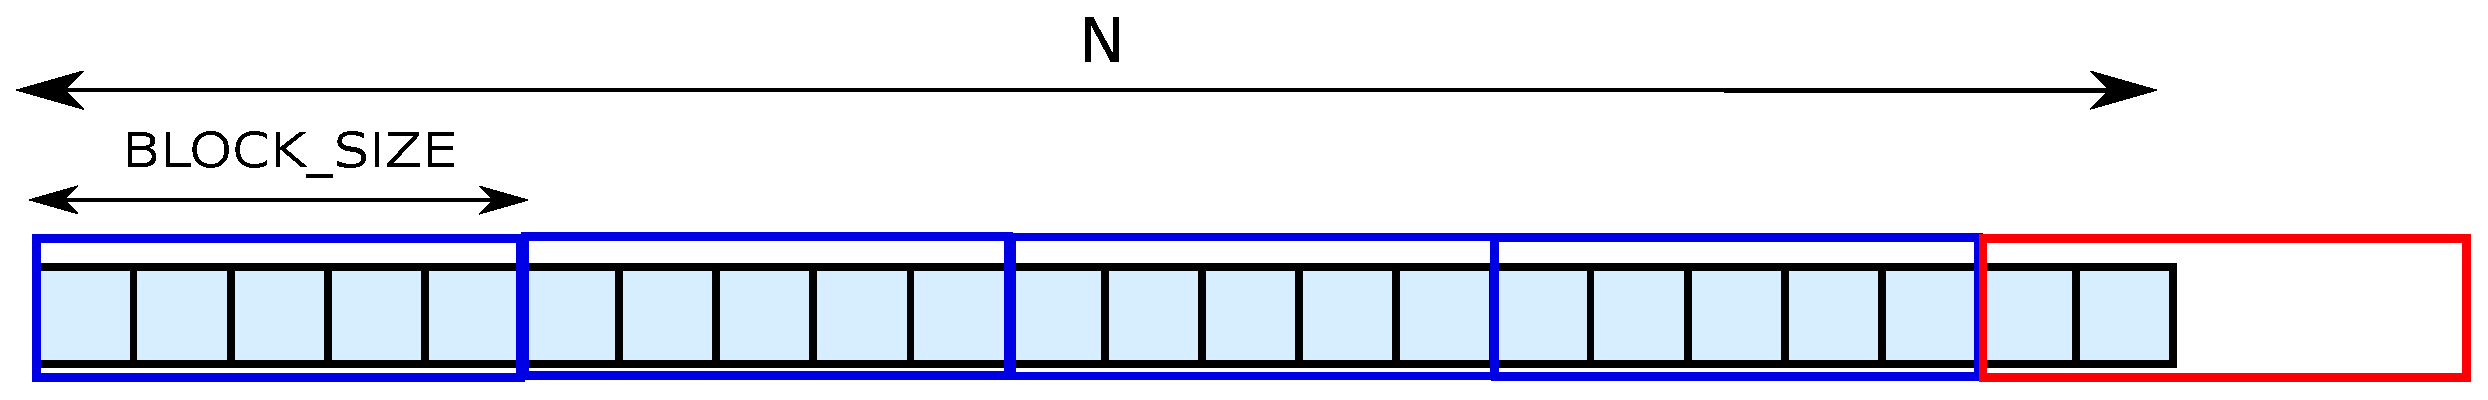
\includegraphics[width=0.7\linewidth]{fig/grille_1D.eps}
\end{center}
   \item[\egia] \texttt{\small currentIndex = blockDim.x * blockIdx.x + threadIdx.x}
   \item[\kontuz] penser à vérifier que \texttt{currentIndex} $\leq$ N !
 \end{itemize}
  \end{itemize}
\end{frame}
%****************************************************************
% Tailles des grilles/blocs
%****************************************************************
\begin{frame}{Taille de blocs}{Exemple XOR}
\begin{flushright}
\includegraphics[width=0.1\linewidth]{fig/xor.jpg}
\end{flushright}
  \lstinputlisting[language=C]{code/overflow.cu}
\end{frame}
%****************************************************************
% Coalescence
%****************************************************************
\begin{frame}{Coalescence}
  \begin{itemize}[<+->]
    \item chaîne (warp) permet jusqu'à 32 accès mémoire concurrents
    \item un accès mémoire typique $\thicksim$ 4 octets
    \item granularité mémorielle : de 32 à 128 octets 
    \item[\argi] {\em coalescence} : agrégation de plusieurs accès mémoire en un seul lorsqu'il se font dans le même bloc
   \item exemples avec 4 threads par chaîne et 4 mots par transaction
\begin{center}
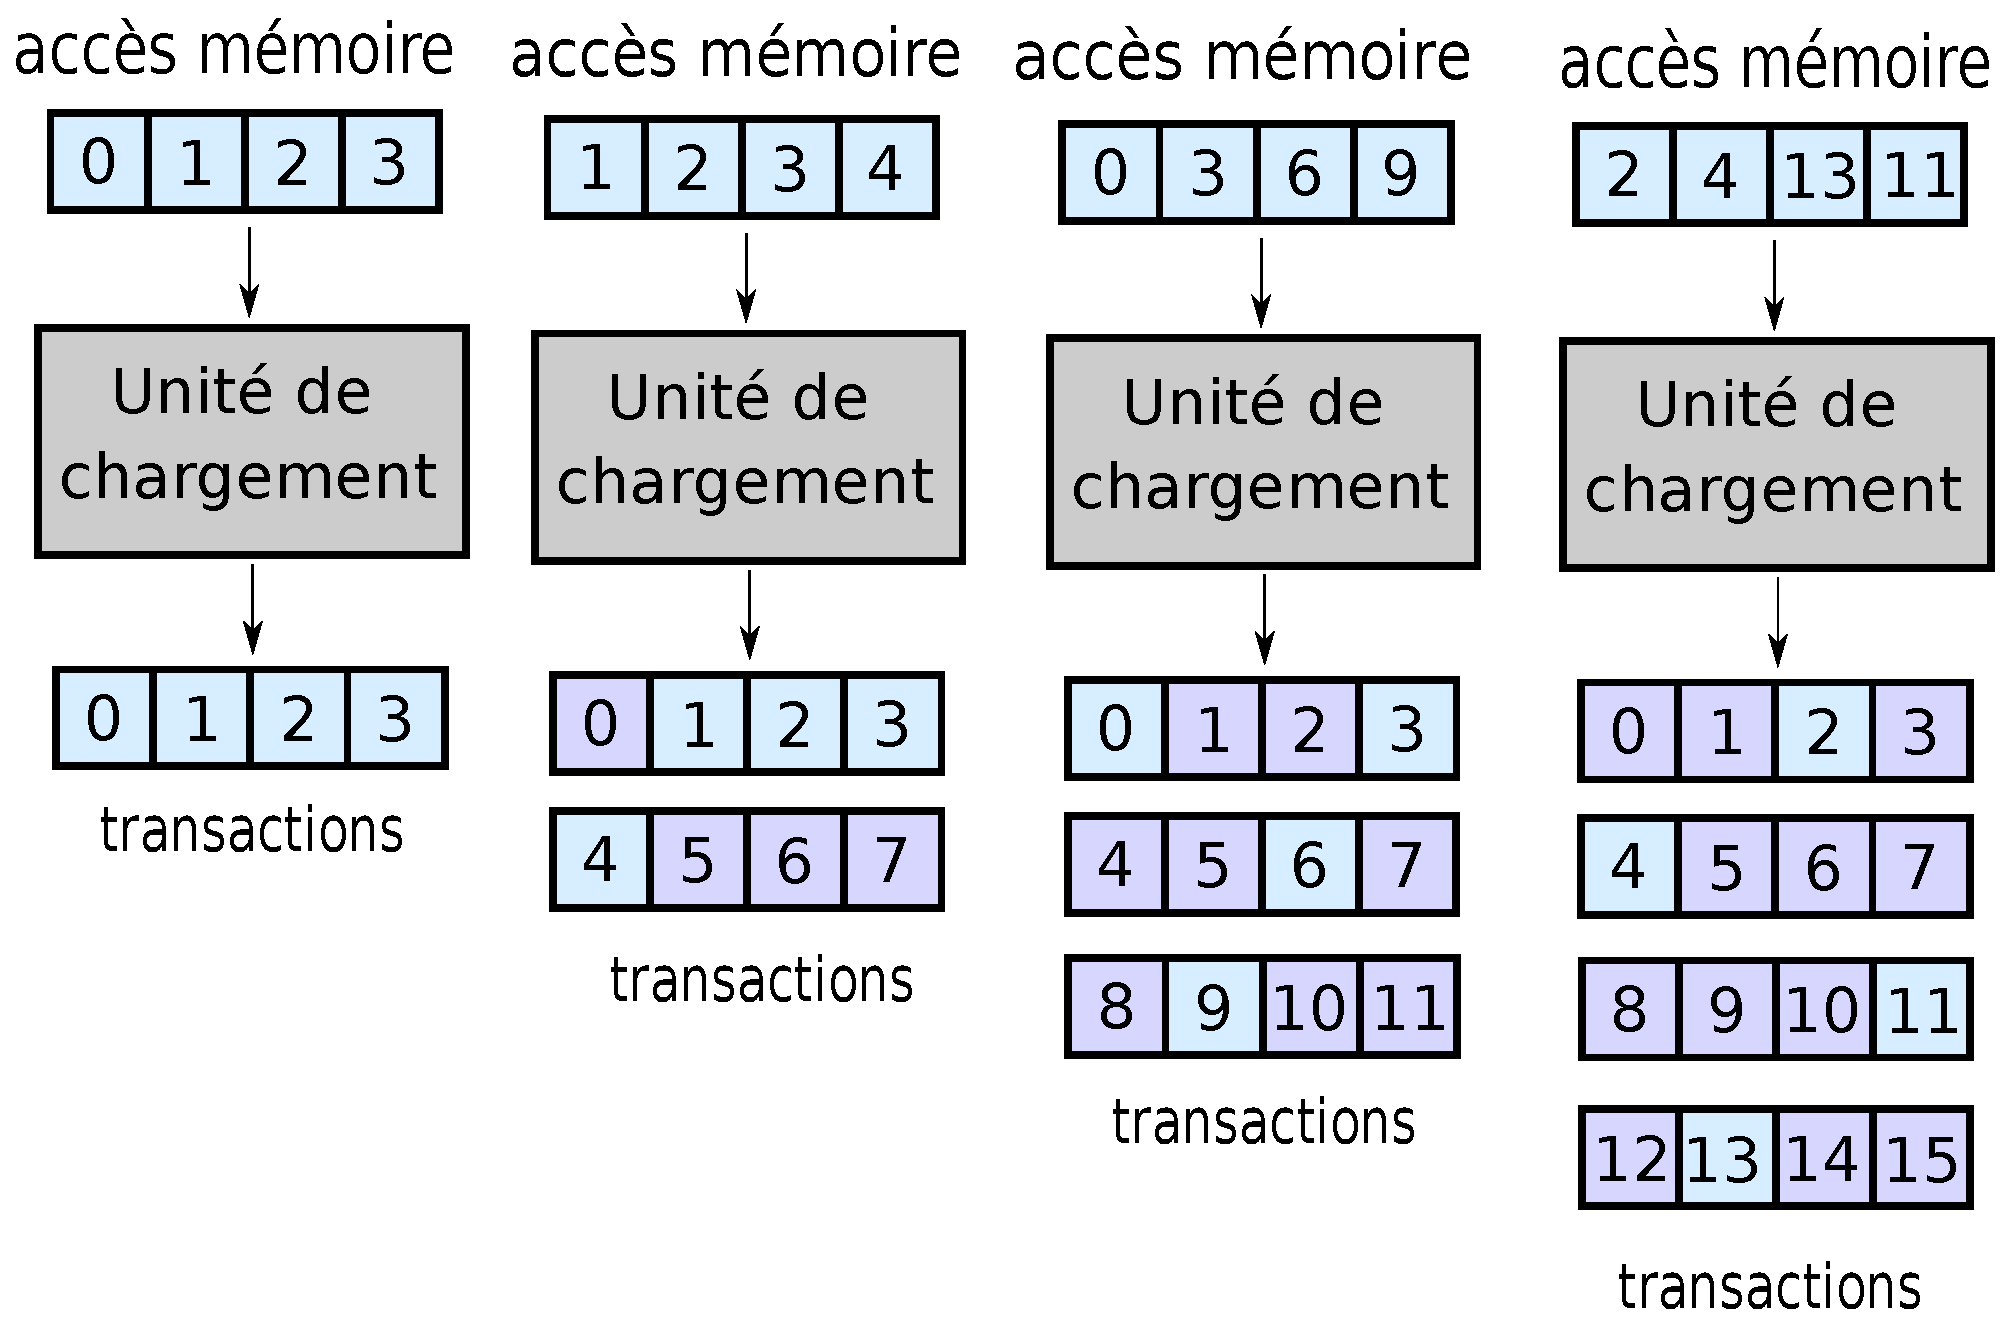
\includegraphics[width=0.6\linewidth]{fig/coalescence.eps}
\end{center}
  \end{itemize}
\end{frame}
%****************************************************************
% References
%****************************************************************
\begin{frame}{Références}
\begin{itemize}[<+->]
  \item[\Pdf] Programming GPU Accelerators with OpenCL, R. Namyst, P.-A. Wacrenier \href{https://raymond-namyst.emi.u-bordeaux.fr/ens/pap/PAP-GPU.pdf}{\beamergotobutton{pdf}}
  \item[\liburu] Cuda Fortran for Scientists and Engineers, G. Ruetsch, M. Fatica
  \item[\Pdf] Understanding Latency Hiding on GPUs, V. Volkov \href{http://www2.eecs.berkeley.edu/Pubs/TechRpts/2016/EECS-2016-143.pdf}{\beamergotobutton{pdf}}
  \item[\faFilePowerpointO] CUDA Basics, S. Vialle \href{http://www.metz.supelec.fr/metz/personnel/vialle/course/PPS-5A-GPGPU/notes-de-cours-specifiques/PPS-GPU-02-CUDA-Basics-2spp.pdf}{\beamergotobutton{pdf}}
\end{itemize}
\end{frame}
\end{document}
